\section{Sprint Retrospective}
El estado del TP entregado no es lo esperado ni lo solicitado, por lo que se torna difícil realizar conclusiones de cierre sobre algo que no cumple con esa condición, estar terminado. 

No se pudieron apreciar por completo las bondades ni dificultades de la metodología scrum porque decir que se siguió a rajatabla (dentro de la flexibilidad que ofrece) la metodología es una mentira. La dinámica del grupo no fue la esperada, con algunos desencuentros entre los integrantes, lo que dificultó considerablemente la tarea de llevar a cabo un desarrollo exitoso.
Esta situación se refleja claramanete en el resultado final de nuestro burndown chart:

\begin{center}
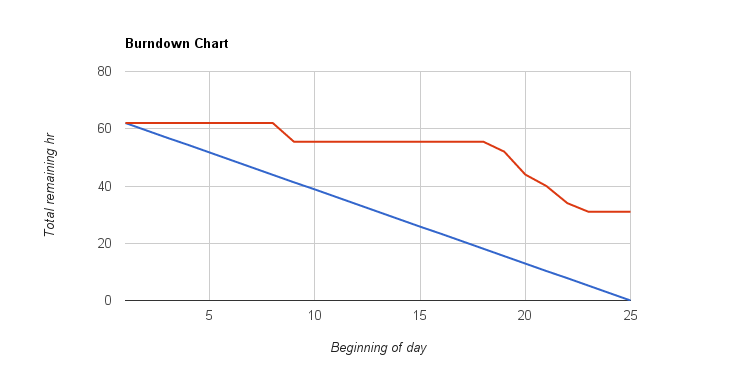
\includegraphics[scale=0.4]{burndown.png} 
\end{center}

Algunos comentarios concernientes a la metodología que se podrían hacer son los siguientes:
\begin{itemize}
 \item Se sobreestimó la cantidad de horas que podría dedicarle cada integrante al grupo; si bien creimos que pusimos un número bastante conservador, ni siquiera se llegó a cumplir esa dedicación para el Trabajo Práctico. 
 \item Se subestimó la cantidad de horas para algunas tareas. No hay tareas que puedan llevar 0.5hrs, y muy pocas tareas que puedan llevar 1 hora. 
 \item Entre los dos items anteriores está claro cuán alejada estuvo finalmente la estimación de la realidad, y además, que en ambos puntos nos equivocamos en direcciones opuestas, aumentando aún más la famosa brecha.
 \item En base a lo vivido en el sprint, Scrum pareciera tener más sentido para un grupo reducido de personas que está cotidianamente en el mismo lugar, dedicándole una cantidad de horas similar a las tareas, y con una comunicación fluida y constante. La flexibilidad es una ventaja cuando se es dinámico y se tiene una adaptabilidad rápida a las distintas situaciones y problemáticas que van surgiendo a lo largo del desarrollo. De ser esta conjetura cierta, el grupo no respetó bien ninguno de los puntos, y la falta de dinamismo e ida y vuelta ocasionó que no se pudieran tomar las decisiones necesarias en el momento indicado, retrasando todo.
 \item Es bastante difícil entrar en contacto con una metodología completamente desconocida para los integrantes en apenas unas semanas, y en el marco de una materia, donde además hay otras responsabilidades (relacionadas con la materia, con la Facultad, y las peores de todas, las ajenas a todo ello).
\end{itemize}


